%!TEX root=bare_conf.tex
\section{Approach}\label{sec:approach}
Similar to the CFG based static analysis, our approach also first constructs a detection model of C program, where memory leak may happen. The main difference of our approach is that, we perform projection in constructing the detection model, which simplifies the later memory leak detection procedure based on the model.

\subsection{Projection Algorithm}

This section describes a set of rules and an algorithm for projecting a control flow graph to a simply one. First of all, we introduce several concepts. These are going to be used in the projection rules.

%\begin{definition}[Projection Subject]
%Projection subject is the control flow graph of the program to be analyzed, which is a directed graph $G=(N, E)$, where $N = \{n_1, n_2, \ldots, n_k\}$ denotes the set of nodes, and $E = \{e_1, e_2, \ldots, e_k\}$ denotes the set of edges. In the procedure $P$, each statement is a node $n$, and there is an edge $e$ between two statements executed in sequence. 
%\end{definition}

$Projection Subject$ is the input of the projection process and $Projection Target$ is the output of the projection process. Specifically, $Projection Subject$($G$) is the control flow graph of the program to be analyzed. $G=(N, E)$, where $N = \{n_1, n_2, \ldots, n_k\}$ denotes the set of nodes, and $E = \{e_1, e_2, \ldots, e_k\}$ denotes the set of edges. In the procedure $P$, each statement is a node $n$, and there is an edge $e$ between two statements executed in sequence. $Projection Target$($G^*$ ) is a directed graph that contains all the control flow branch nodes denoted by $B$, and all the allocation nodes denoted by $A$ and deallocation nodes denoted by $F$ (if exist). $G^* = (N^*, E^*)$, where $N^* = A\cup B\cup F$ ($A\cap B\cap F=\emptyset$) denotes the set of nodes, and $E^*$ denotes the set of edges between nodes, representing the sequential ordering between nodes.

%\begin{definition}[Projection Target]
%Projection target is a directed graph $G^*$ that contains all the control flow branch nodes denoted by $B$, and all the allocation nodes denoted by $A$ and deallocation nodes denoted by $F$ (if exist). $G^* = (N^*, E^*)$, where $N^* = A\cup B\cup F$ ($A\cap B\cap F=\emptyset$) denotes the set of nodes, and $E^*$ denotes the set of edges between nodes, representing the sequential ordering between nodes.
%\end{definition}

\begin{definition}[Control Flow Graph Projection]
Given two directed graphs $G = (N, E)$ and $G^* = (N^*, E^*)$. Let set $M$ contains all the statement nodes relating to memory management in the procedure $P$ and the set $B$ contains all the control flow branch nodes (e.g. {\sf if}, {\sf else}, {\sf while}, {\sf for} et al.). If $G$ and $G^*$ satisfy the following conditions, then we say that $G^*$ is the projection of $G$, denoted as $G^* \mapsto G$:
\begin{itemize}
\item
$N^*\subseteq N$;
\item
If $\forall m,n\in N^*,(m\neq n), if m\in \Gamma(n)$ ($\Gamma(n)$ denotes the set of direct successor nodes of $n$), then there must be a connected path $\mu$ from $n$ to $m$ in $G$, formally $\exists \mu=(n, n_1,\ldots,n_l,m)$ in $G$ and $n_1\in\Gamma(n) \land  n_{i+1}\in\Gamma(n_i) \land n_n\in \Gamma(m)$ ($0\leq i\leq (n-1)$);
\item
$\forall$ $n\in B$ in directed graph $G^*$, if $\forall m\in M: m\not\in \Gamma(n)$, then $\Gamma(n)=\Gamma(n)\cup\{n\}$. 
\end{itemize}
\end{definition}

In general, the \emph{Control Flow Graph Projection} is the process from the \emph{Projection Subject} transforming into the \emph{Projection Target} according to the following rules, we summarize the projection rules as follows: 
\begin{itemize}
\item 
Rule 1: The set $N^*$ of the projection graph only contains nodes related to memory allocation and deallocation, and all the control flow branch nodes in the procedure $P$.
\item
Rule 2: If a control flow branch contains the nodes related to memory allocation and deallocation, then the nodes that related to memory allocation and deallocation will be the successor nodes of this branch node in the projection graph $G^*$.
\item
Rule 3: If a control flow branch does not contain direct successor nodes that related to memory allocation and deallocation, then this branch node will form a closed node in the projection graph $G^*$. 
If the node $n\in N^*$, $n\in \Gamma(n)$, then the node $n$ is a closed node.
\end{itemize}


% that is, the degree of the branch node plus one.

Fig.~\ref{fig:3} shows the CFG (G) of a piece of code. In this graph, there are $11$ elements forms set $N$, that is, $N = \{S_0, S_1, S_2, S_3, S_4, S_5, S_6, S_7, S_8, S_9, S_{10}\}$. The memory block is allocated in $S_1$ ($S_1\in A$) and freed in $S_9$ ($S_9\in F$); $S_3$ is a looping branch node and $S_6$ is a conditional branch node ($B=\{S_3, S_6\}$); In node $S_7$, another pointer points to the memory block ($S_7\in A$); Others are unrelated to memory operation. Thus the cyclomatic complexity of this graph is $4$.
Fig.~\ref{fig:4} shows the projection graph $(G^*)$ of $G$. Following the projection Rule 2, we have $N*=A\cup B\cup F=\{S_1, S_3, S_6, S_7, S_9\}$. Following Rule $2$, we have the edges from $S_1$ to $S_3$, $S_3$ to $S_6$, $S_6$ to $S_7$ and $S_7$ to $S_9$. Following Rule $3$, $S_3$ is a closed node since all its direct successor nodes are not memory related nodes, thus we add a loop to $S_3$. There is no loop at $S_6$, because the direct successor $s_7$ is a memory related node.  

\begin{figure}[!h]
\center
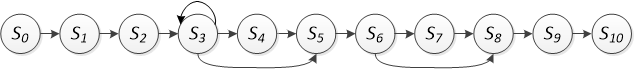
\includegraphics[width=0.5\textwidth]{figure/fig1-fig4/fig_3}
\caption{The CFG of the program (G)}
\label{fig:3}
\end{figure}

\begin{figure}[!h]
\center
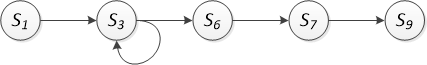
\includegraphics[width=0.35\textwidth]{figure/fig1-fig4/fig_4}
\caption{The projection graph (G*)}
\label{fig:4}
\end{figure}

\begin{theorem}[Control Flow Graph Projection Theorem]
Given a directed graph $G = (N, E)$. If $G^* \mapsto G$ where $G^*=(N^*, E^*)$, then $G^*$ strictly keeps the reachability relation among nodes in $N^*$ from $G$, that is, $\forall m,n\in N^*$, $m$ can reach $n$ in $G^*$ if and only if $m$ can reach $n$ in $G$.
\end{theorem}

\begin{proof} Presume $m$ can reach $n$ in $G^*$, which means there exists a directed path $\mu^*=(m,e_1^*,e_2^*,\ldots,e_k^*,n)$ in $G^*$. 
Since $G^* \mapsto G$, then there must exist a set of paths $\mu_0=(m,e^0_i,\ldots,e^0_{j_0}, e_1^*)$, $\mu_i=(e^*_{i}, e^{i}_i,\ldots,e^{i}_{j_i}, e_{i+1}^*)$ ($1\leq i\leq k-1$) and $\mu_k=(e_k^*,e^k_i,\ldots,e^k_j, e_{j_k}, n)$ in $G$, where $e^{i}_{j_i}$ can be empty. The $k$ paths are connected since the last node in a path is the starting node of another path. Formally, given path $\mu_i=(e^*_{i}, e^{i}_i,\ldots,e^{i}_{j_i}, e_{i+1}^*)$ and $\mu_{i+1}=(e^*_{i+1}, e^{i+1}_{i+1},\ldots,e^{i+1}_{j_{i+1}}, e_{i+2}^*)$. According to the definition of path, we have $e_{i+1}^*\in \Gamma(e^{i}_{j_i})$ in path $\mu_i$
and $e^{i+1}_{i+1} \in \Gamma(e^*_{i+1})$ in path $\mu_{i+1}$. Thus we have a path from $e^{i}_{j_i}$ to $e^{i+1}_{i+1}$ via $e^*_{i+1}$. That is we can connect $\mu_i$ and $\mu_{i+1}$ as path $(e^*_{i},e^{i}_i,\ldots,e^{i}_{j_i}, e_{i+1}^*, e^{i+1}_{i+1},\ldots,e^{i+1}_{j_{i+1}}, e_{i+2}^*)$. In this way, by connecting the $k$ paths, we have a path from $m$ to $n$ in $G$.
%At the same time, then there must exist $\mu=(e_j^*,\ldots,e_t^*)\in G$ for $e_j^*, e_t^*\in μ^* (1\leq j<t\leq k)$ , $e_t^*\in \Gamma(e_j^*)$. So on and so forth, the directed path $\mu=(n,\ldots,m)\in G$ can be deduced, that is $m$ can reach $n$ in $G$. 

On the other hand, presume $m$ can reach $n$ in $G$, that is there exists a directed path $\mu=(m,\ldots,n)$ in $G$, then there must be:
\begin{itemize}
\item
Either there are no other nodes in $N^*$ except $m$ and $n$; 
\item
Or there is $\mu=(m,\ldots,n_1,\ldots,n_2,\ldots,n_k,\ldots,n)$, where $m$, $n$, $n_i\in N^* (1\leq i \leq k)$, and the remaining nodes do not belong to $N^*$.
\end{itemize}
%
In the former case, according to the rules of control flow graph projection, $m$ can immediately reach $n$ in $G^*$, i.e., $n\in \Gamma(m)$.
%
In the later case, let $\mu=m,\mu_1,n_1\mu_2, n_2,\cdots,\mu_k, n_k, \mu_{k+1}, n$, where $\mu_i=(n^i_{1},\ldots,n^i_{j_i}) (1\leq i\leq k+1)$, there are no nodes in each path $\mu_i$ from $N^*$ except end nodes. According to the projection rules, the nodes in each path $\mu_i$ will be deleted in $G^*$ such that there is a immediate edge between $m$ and $n_1$, between each $n_i$ and $n_{i+1} (1\leq i \leq k)$, and between $n_{k+1}$ and $n$, which forms a path $
\mu^*=(m, n_1, n_2, \ldots, n_{i}, n_{i+1}, \ldots, n_{k+1}, n)$ in $G^*$. 
\end{proof}

Algorithm~\ref{alg:cfp} shows the projection algorithm according to the projection rules. %We can summarize from the control flow graph projection theorem that $G^*$ is a directed graph extracted from $G$ which consists of $N^*$. Apart from this, $G^*$ strictly keeps the reachable relationships among nodes in $N^*$ from $G$. Specifically, if $N^* = N$, then $P[G, N^*] = G$.
%
Given the control flow graph $G = (N, E)$ of program $P$ as input. The algorithm returns $G$'s projection graph $G^*= (N^*, E^*)$ as output. Algorithm 1 can be divided into $3$ steps. Step$1$(line $1-2$) establishes the min-heap of $N$ according to the execution order of statements. Step$2$(line $3-9$) folds those unrelating to memory management paths. Step$3$(line $10-12$) adjusts the $\mathit{Red\_Black\_Tree}(N^*)$ and the $\mathit{Map}(N^*)$, and obtains the final projection graph $G^*$).
% and $G^*=P[G, N^*]$. $N^* = A\cup B\cup F$. Moreover, 
In this algorithm, $n.ind$ and $n.outd$ stand for the in-degree and out-degree of node $n$ respectively. $A.a$ means the node $a$ is in set $A$. $F.f$ means the node $f$ is in $F$. Lastly, whenever a loop is added to $G^*$ (even when the loop already exists), both the in-degree and the out-degree of the looping node are increased by one.

%The set $N$ contains all the nodes abstracted from the statements from procedure $P$. 
Considering the complexity of the projection algorithm, the Red Black Tree is used to store the nodes in set $N$. Red Black Tree is a data structure, which is an approximate balanced tree with only two types of nodes: red nodes and black nodes. This type of data structure has the advantage of high search efficiency, due to that it is sequential which can avoid the disorder during the search process. 

In the algorithm, the set $E$ in graph $G$ (the execution sequence of statements in procedure $P$) is implemented as a set of $Map$s. A $Map$ is a data structure stored in the form of key-value pairs. The elements in a $Map$ are the ordering relation between a node $n$ in set $N$ and its successor nodes (i.e., nodes in $\Gamma(n)$).

\begin{algorithm}
\caption{ControlFlowProjection ($G$)}\label{alg:cfp}
\textbf{Input:} A control flow graph $G$ for program $P$.\\
\textbf{Output:} Projection graph $G^*$ for the input control flow graph\\
%\textbf{Begin}\\
%Step1: (According to the execution order of statements, establish the min-heap of $N$)\\
1.\quad	Initialize the Red Black Tree $\mathit{Red\_Black\_Tree}(N)$.\\
%2.\quad	\textbf{init} $\mathit{Red\_Black\_Tree}(N)$;\\
%3.\quad	\textbf{create} $\mathit{Red\_Black\_Tree}(N)$;\\
%2.\quad	$\forall n\in N, \mathit{Map}(n)\leftarrow(n,\Gamma(n))$;\\
2.\quad	For all $n$ from $N$, add $n$ and $\Gamma(n)$ to $\mathit{Map}(n)$.\\
%Step2: (Fold paths)\\
3.\quad	\textbf{while} $\mathit{Red\_Black\_Tree}$.hasNext \textbf{do}\\
%4.\quad	\textbf{do}\\
4.\quad	\textbf{if} $n.ind\geq 2 || n.outd\geq 2$ \textbf{then}\\
5.\quad \quad    \textbf{if} $A.a\in \Gamma(n) || F.f\in \Gamma(n)$\\
6.\quad \quad	    \textbf{then} $\Gamma(n)\leftarrow A.a || \Gamma(n)\leftarrow F.f$\\
7.\quad	\textbf{else} \\
8.\quad \quad   \textbf{then} $\Gamma(n)\leftarrow (n\cup \Gamma(n)\cap N^*)$\\
9.\quad\textbf{end}\\
%Step3: (Adjust the $\mathit{Red\_Black\_Tree}(N^*)$ and the $\mathit{Map}(N^*)$, and obtain the final projection graph $G^*$)\\
10.\quad	Delete all $n$ that are not in $N^*$.\\
11.\quad	$\mathit{Red\_Black\_Tree(N)} \leftarrow \mathit{Red\_Black\_Tree}(N^*)$.\\
12.\quad	$\mathit{Map}(N) \leftarrow \mathit{Map}(N^*)$.\\
%\textbf{End}
\end{algorithm}

The projection algorithm is acceptable in the aspect of complexity. In this algorithm, we assume that the number of edges is linear in N, all the time complexity of Step1, Step2 and Step3 are $O(log(N))$, and the space complexity of the three steps are $S(N)$($S(N)$ is linear). Therefore, the time complexity of this algorithm is $O(log(N))$ and the space complexity of this algorithm is $S(N)$.

\subsection{Detection Method}

%$G^* \mapsto G$, and $G^*$ is the projection graph of the control flow graph $G$, and there are two definitions on $G^*$.
Given a graph $G^*=(N^*, E^*)$, we define the direct predecessor of a node as follows:

\begin{definition}{Direct Predecessor Node}
For two nodes $m$, $n$ ($m, n\in N^*$), if $m$ is the first open node among all the predecessor nodes of node $n$ (i.e., $Η(n)$), then $m$ is called the direct predecessor node of $n$.
\end{definition}

The detection algorithm (Algorithm~\ref{alg:mld}) takes the output of the projection process as input. %In this paper, stack elimination\footnote{Eliminating Frame Pointer and Arg Pointer. http://gcc.gnu.org/onlinedocs/gccint/Elimination.html. 2017.} is leveraged to detect memory leaks in source code. Algorithm~\ref{alg:mld} shows the detection algorithm, 
Given the nodes in set $A$ or $F$, the algorithm finds the direct predecessor node of all nodes by traversing the Red Black Tree. In this algorithm, the node $base$ is the last node in set $A$ or $F$ traversed to, i.e., $base$ is the currently visiting node. In line $7-12$, the first node from $A$ or $F$ will be pushed into the stack when the stack is empty. Otherwise it traverse the next node. In line $14-20$, there may be memory leaks when the direct predecessor node of $base$ is the node from $B$, according to the second case from Fig.~\ref{fig:1} in Section~\ref{sec:description}. Another situation is that the direct predecessor node of base is not the node from $B$, if the stack is not empty after the detection process, then there may be some memory spaces that have not been freed which may lead to memory leaks.

\begin{algorithm}
\caption{MemoryLeakDetection ($G^*$)}\label{alg:mld}
\textbf{Input:} The projection graph $G^*$.\\
\textbf{Output:} The detection results for memory leaks ($\mathit{true}$ or $\mathit{false}$)\\
%\textbf{Begin}\\
1.\ \	Declare a $\mathit{stack}$ to be detected.\\
2.\ \ 	Declare node $\mathit{base}$ and node $\mathit{current}$ for traverse.\\
3.\ \       \textbf{bool} $\mathit{MemLeak\_Check}$(Tree $\mathit{Red\_Black\_Tree}$, Set $\mathit{Map}$)\\
4.\ \ 	\textbf{while} $\mathit{Red\_Black\_Tree}$.hasNext \textbf{do} \\
%5.\ \ 	\textbf{do begin}\\
5.\ \ \quad	    $\mathit{base} \leftarrow$ null.\\
6.\ \quad	    $\mathit{current} = \mathit{Red\_Black\_Tree}$.$\mathit{current\_Ele}$\\
7.\ \ \quad	    \textbf{if} $\mathit{base}$ == null \textbf{then}\\
8.\ \ \quad\quad	        \textbf{if} $\mathit{current}$ != $A$ \&\& $\mathit{current}$ != $F$ \textbf{then}\\
9.\ \ \quad\quad\quad	            \textbf{continue}\\
10.\ \ \quad\quad	        \textbf{else then}\\
11.\ \ \quad\quad\quad	            $\mathit{base} \leftarrow \mathit{current}$\\
12.\ \ \quad\quad\quad	            $\mathit{stack}$.push($\mathit{base}$)\\
13.\ \ \quad	    \textbf{else then}\\
14.\ \ \quad\quad       \textbf{if} $\mathit{current}\in B$ \textbf{then}\\
15.\ \ \quad\quad\quad            \textbf{if} $B.ind<2 || B.outd<2$ \textbf{then}\\
16.\ \ \quad\quad\quad\quad	                \textbf{return} $\mathit{false}$\\
17.\ \ \quad\quad\quad        \textbf{else if} $\mathit{current} == \mathit{base}$ \textbf{then}\\
18.\ \ \quad\quad\quad\quad	            $\mathit{stack}$.push($\mathit{current}$);\\
19.\ \ \quad\quad\quad	        \textbf{else if} $\mathit{current}$ != $\mathit{base}$ \textbf{then}\\
20.\ \ \quad\quad\quad\quad	            $\mathit{stack}$.pop()\\
21.\ \ 	\textbf{end}\\
22.\ \ 	\textbf{if} $\mathit{stack}$ != null \textbf{then}\\
23.\ \ \quad    \textbf{return} $\mathit{false}$\\
24.\ \ 	\textbf{else then}\\
25.\ \ \quad	    \textbf{return} $\mathit{true}$\\
%\textbf{End}
\end{algorithm}

There are only one loop in the traversal of Red Black Tree, so the time complexity of this algorithm is $O(log(N))$, and the space complexity of this algorithm is $S(N)$.

Take projection graph in Fig.~\ref{fig:4} as an example. According to the detection algorithm, the direct predecessor node of node $S_9$ is node $S_7$, and the direct predecessor node of node $S_7$ is node $S_6$, node $S_6$ is a branch node. That is, the memory blocks are freed in the conditional branch of node $6$, which is determined to be a suspected memory leak.

\subsection{Optimization Strategy}

The control flow graph projection makes the detection process simple and intuitive. More importantly, all the cases of memory leaks mentioned in Section~\ref{sec:description} can be detected in the detection algorithm. However, this approach may result in a high false positive rate, since it does not analyze the specific value of conditional predicate in the valuating of control flow branches, which leads to a low sensitivity to data flows. In Fig.~\ref{fig:7}, the statement $5$ will be marked with a $B$ node (control flow branching statement). Apart from this, the example code will be judged to have a suspected memory leak, by using the algorithm above, since the buffer may not be freed in every branch. However, there are no memory leaks in this example. Specifically, the result of the condition is true when analyzing the conditional predicate of line $5$ (buffer != NULL), that is, the memory blocks are freed after being allocated. 

In order to reduce such false positives, this paper combines symbolic execution\footnote{Symbolic execution.https://en.wikipedia.org/wiki/Symbolic\_execution.2017.} and constraint solving\footnote{Constraint solving. http://www.constraintsolving.com/. 2017.} during the execution of the algorithm to accurately evaluate the branching conditions.
%
\begin{figure}[!h]
\small
\center
\begin{lstlisting}[frame=single,framexrightmargin=-10pt,numbers=right] 
void main(){
 long *buffer;
 size_t size;
 buffer= (long*)malloc(1000*sizeof(long));
 size = _msize(buffer);
 if(buffer != NULL)
 free(buffer);
}
\end{lstlisting}
\caption{A piece of code}\label{fig:7}
\end{figure}

Symbolic execution simulates the execution of programs by symbolizing variables. Specifically, symbolic execution collects memory allocation and release points by backward traversal for the CFG. At the same time, at each of the control flow branch, conditions of the branch are added to the current path conditions. Finally, those paths related to memory allocation and release will be merged at the meeting node of the CFG, and then according to Hoare logic\footnote{Hoare logic. https://en.wikipedia.org/wiki/Hoare\_logic. 2017.}, our system carries constraint solving to the merged paths. Constraint solving is accompanied by the projection process.  
%Therefore, symbolic execution and constraint solving can help to reduce similar false positives like the problem in this example.

\subsection{System Workflow}

%\begin{figure}[!h]
%\small
%\centering
%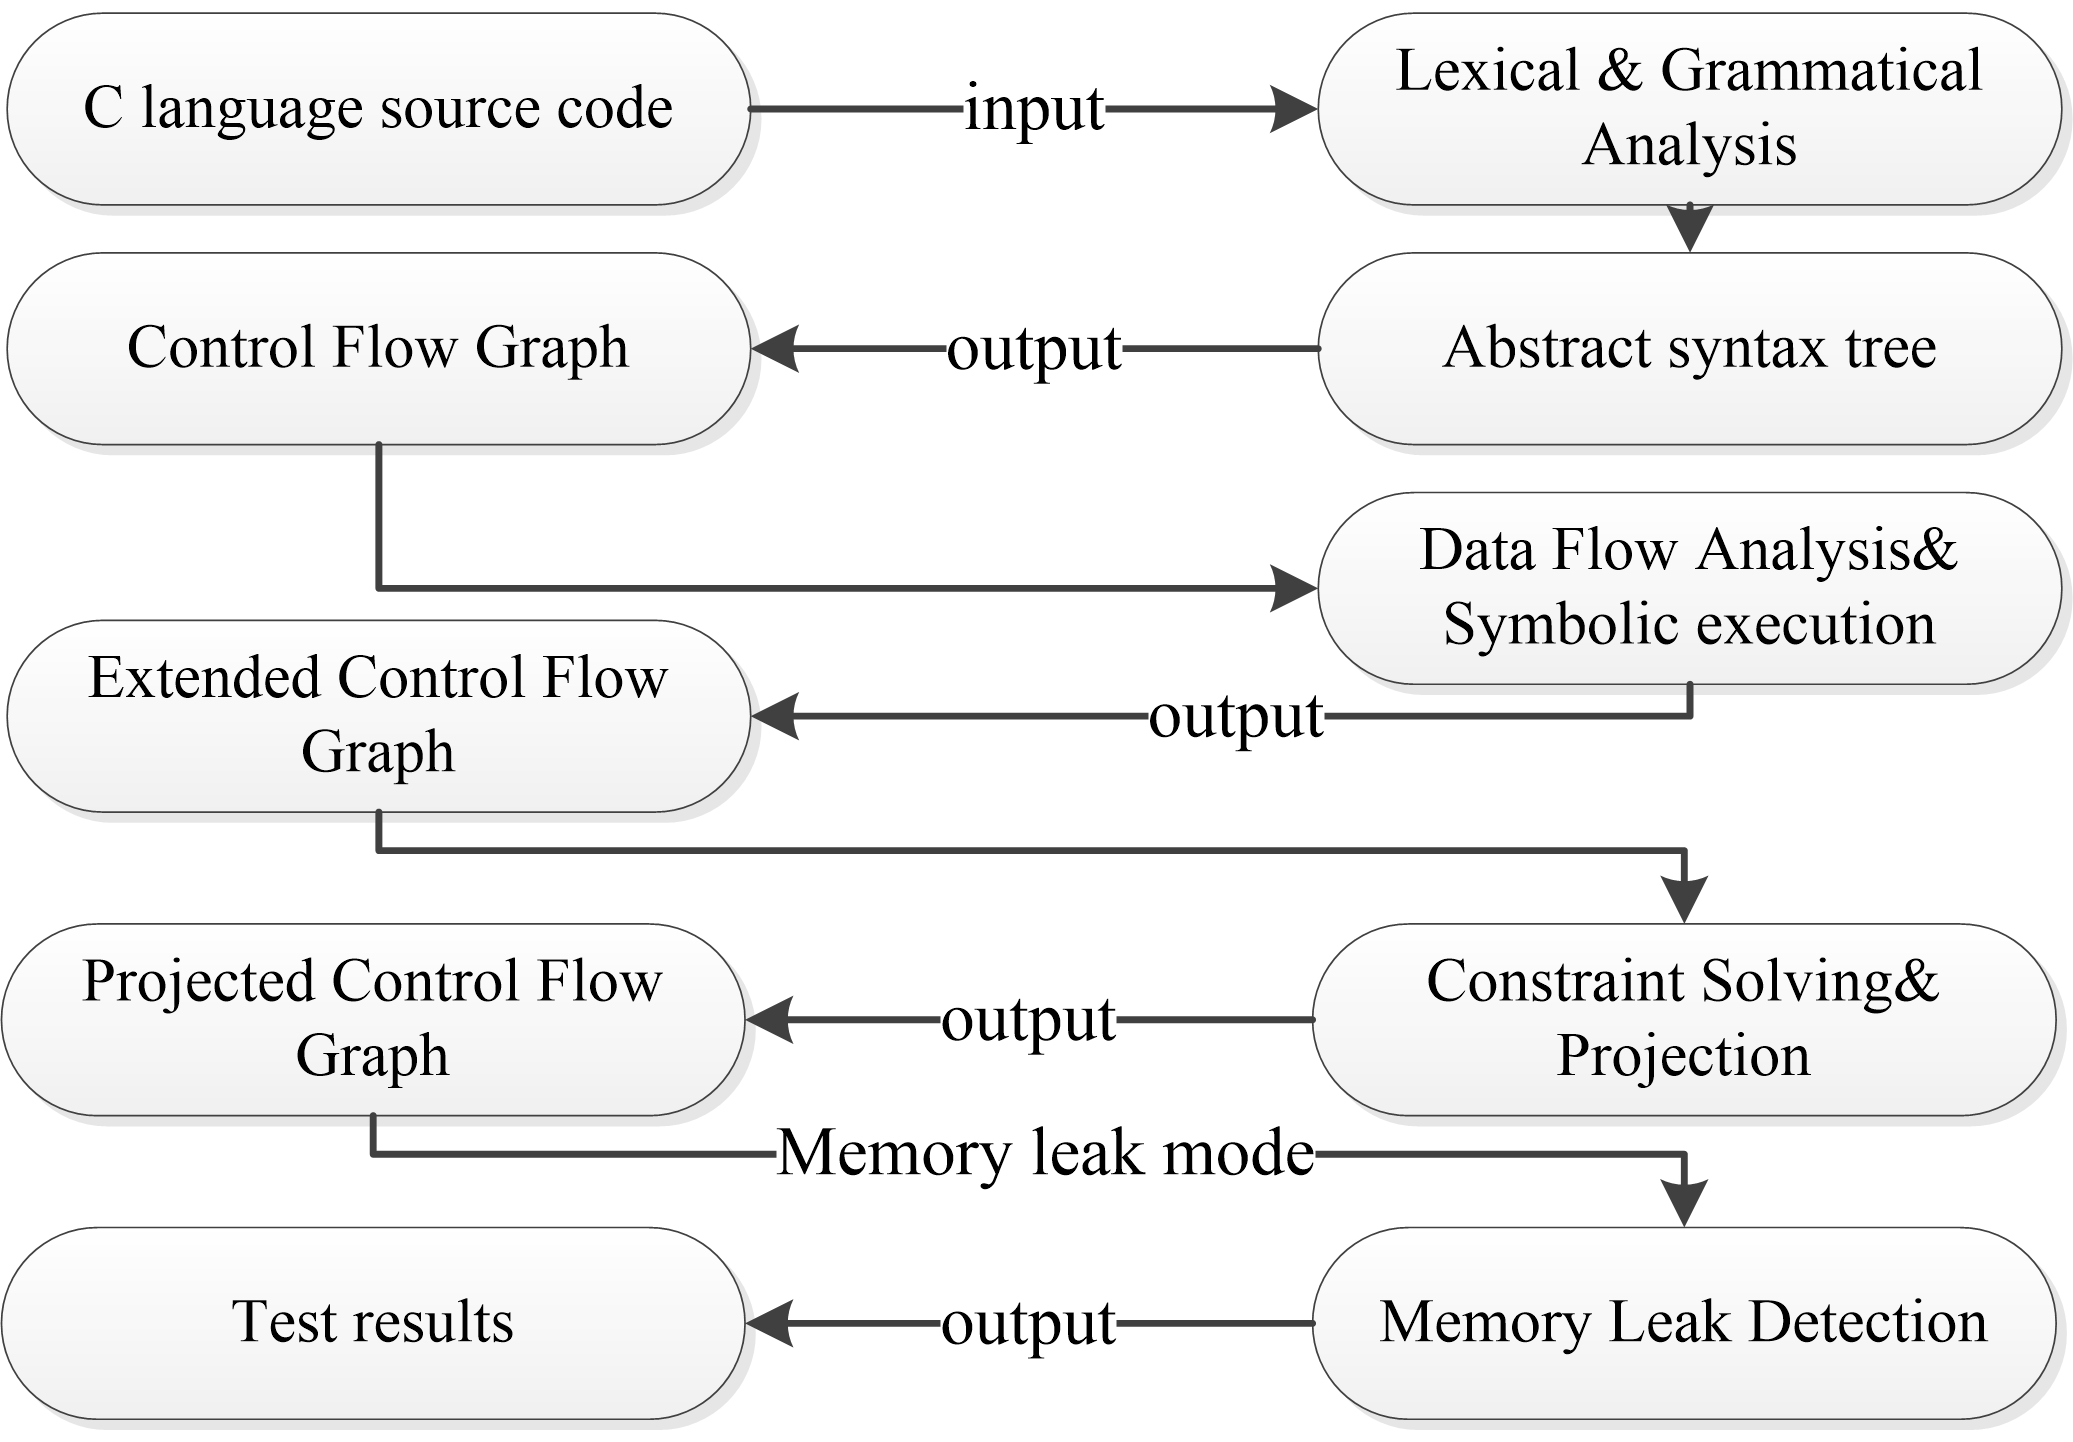
\includegraphics[width=0.5\textwidth]{figure/fig8-fig12/fig_new}
%\caption{Framework flowchart for PML\_Checker}\label{fig:18}
%\end{figure}

The input data of PML\_Checker is C language source code. After lexical analysis and syntax analysis, Abstract syntax tree generates the original control flow graph, which will be output to the system interface. Next, data flow analysis and symbolic execution extend the original CFG, constraint solving to the data flow conditions will find the dependencies from the memory allocation to deallocation, and the extended CFG will be output as a mid product. Then the projected CFG wil be produced at the base of extended CFG by projection algorithm. At last, according to the detection method mentioned at the approach section, PML\_Checker detects memory leaks from the projected CFG, and displays the test results. 

